% day2_seg2_ranproc2/rand_walk.tex
\begin{frame}
  \onslide<1->{
	\frametitle{Some Important Random Processes} 
	\framesubtitle{Random Walk}
}
\begin{itemize}
  \onslide<2->{
 \item In engineering applications, random walk is often considered as a discrete time process.
}
  \onslide<3->{
 \item Some authors (Gelb, for example) refer to continuous-time random walk as the
 solution of a differential equation driven by white noise:
 $\dot{x}=w$.
}
  \onslide<4->{
 \item However, that would require $w$ to be integrable which it is not, because it is not of bounded variation.  
 Alternatively, it would require the Wiener-Levy process to be differentiable, which it is not
}
  \onslide<5->{
 \item So we'll stick to the bandlimited or the discrete case: $x(k+1)=x(k) + w(k)$,
 where the $w(k)$ are normally distributed and statistically uncorrelated at distinct sample times
}
\end{itemize}
\end{frame}

\begin{frame}
  \onslide<1->{
	\frametitle{Some Important Random Processes} 
	\framesubtitle{Random Walk:  Bandlimited White Noise is Integrable}
}
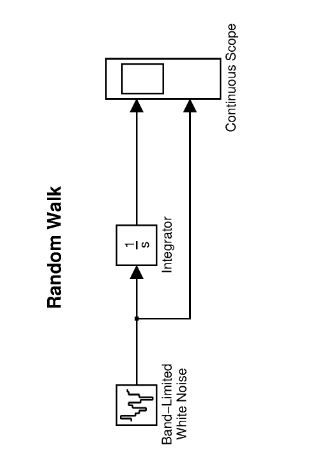
\includegraphics[angle=-90, scale=0.80]{day2_seg2_ranproc2/rand_walk.jpg}
\end{frame}

\begin{frame}
  \onslide<1->{
	\frametitle{Some Important Random Processes} 
	\framesubtitle{Discrete Random Walk}
}
\begin{itemize}
  \onslide<2->{
\item  $x(k)=x(k-1)+w(k)$, where $w(k)$ is a white sequence 
}
  \onslide<3->{
\item  Another way of looking at this is to say that the difference sequence is white:  $x(k)-x(k-1)=w(k)$ 
}
  \onslide<4->{
\item  In MATLAB you can use the diff function to create the difference sequence from a give sequence. Note that 
it would have 1 less element than the original sequence:\\
x=rand(1,5); dx=diff(x);\\
x =    [ 1,     0,     2,    -1,     4]\\
dx =  [-1,     2,    -3,     5] 
}
\end{itemize}
\end{frame}

\begin{frame}
  \onslide<1->{
	\frametitle{Some Important Random Processes} 
	\framesubtitle{Discrete Random Walk:  Raytheon Stock Price (4000 daily samples)}
}
\begin{center}
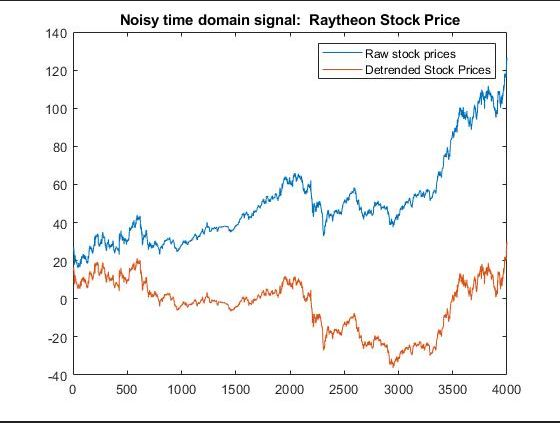
\includegraphics[scale=0.50]{day2_seg2_ranproc2/rtn_stock_prices.jpg}
\end{center}
\end{frame}
 
\begin{frame}
  \onslide<1->{
	\frametitle{Some Important Random Processes} 
	\framesubtitle{Discrete Random Walk:  Raytheon Stock Price Power Spectal Density}
}
\begin{center}
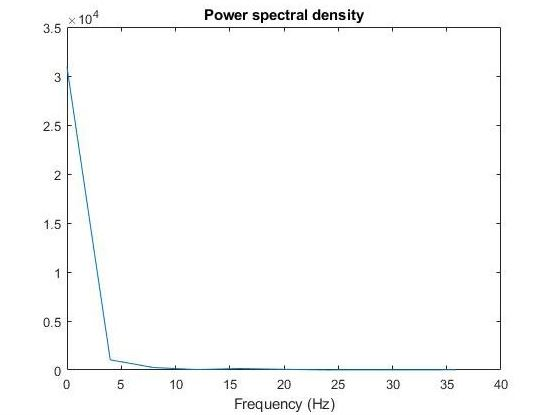
\includegraphics[scale=0.50]{day2_seg2_ranproc2/rtn_randwalk.jpg}
\end{center}
\end{frame}

\begin{frame}
  \onslide<1->{
	\frametitle{Some Important Random Processes} 
	\framesubtitle{Discrete Random Walk:  Detrened Difference of Raytheon Stock Price}
}
Let's see if the difference sequence of detrended stock prices looks like white noise:
\begin{center}
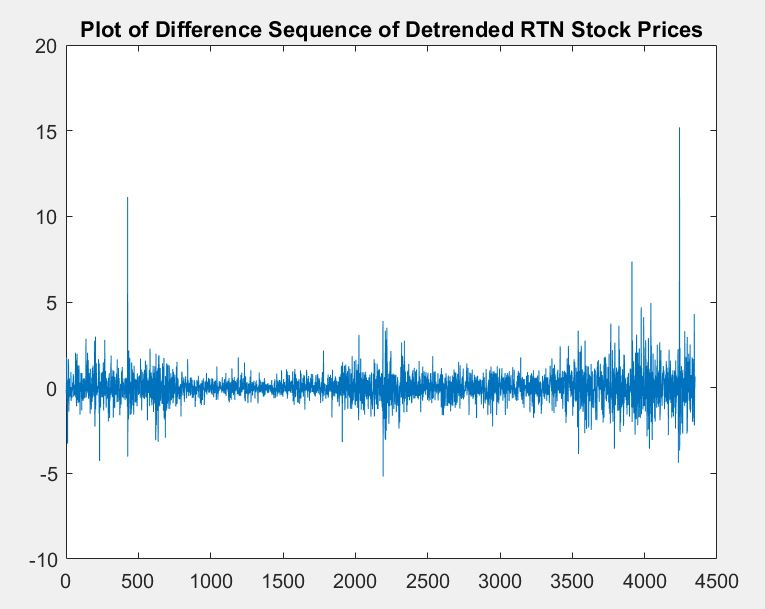
\includegraphics[scale=0.50]{day2_seg2_ranproc2/rtn_stock_prices_diff_detrended.jpg}
\end{center}
\end{frame}
